

\chapter{Método Proposto}
\label{sec:MetodoPrincipal}
O método proposto recebe um quadro $I_{t}$ no instante $t$ e o quadro no instante anterior $I_{t-1}$.
A saída gerada pela arquitetura consiste em um mapa de densidade 2D indicando a localização de cada alevino presente no quadro e a estimativa dos vetores de deslocamento para cada alevino. 

Vide as dificuldades das CNN's em detectar objetos que se movem rapidamente em vídeos (Seção \ref{sec:Motivacao}). Este método recebe informações das cenas anteriores a fim de passar para os ramos de estimativa, a localização e formato do objeto em diversas ocasiões. 

A ordenação metodológica pode ser descrita em quatro passos principais conforme a Figura \ref{fig:model}. Inicialmente, as imagens passam por um pré-processamento (passo 1) para construção do volume de entrada (V). Após isso um mapa de características é obtido para $V$ usando uma CNN (e.g., VGG19\cite{VGG}) (passo 2). O mapa de características é dado como entrada para dois ramos que estimam o mapa de densidade (passo 3) e os vetores de deslocamento (passo 4). As seções abaixo descrevem as etapas em detalhes.

\begin{figure}[!hbt]
	\centering
	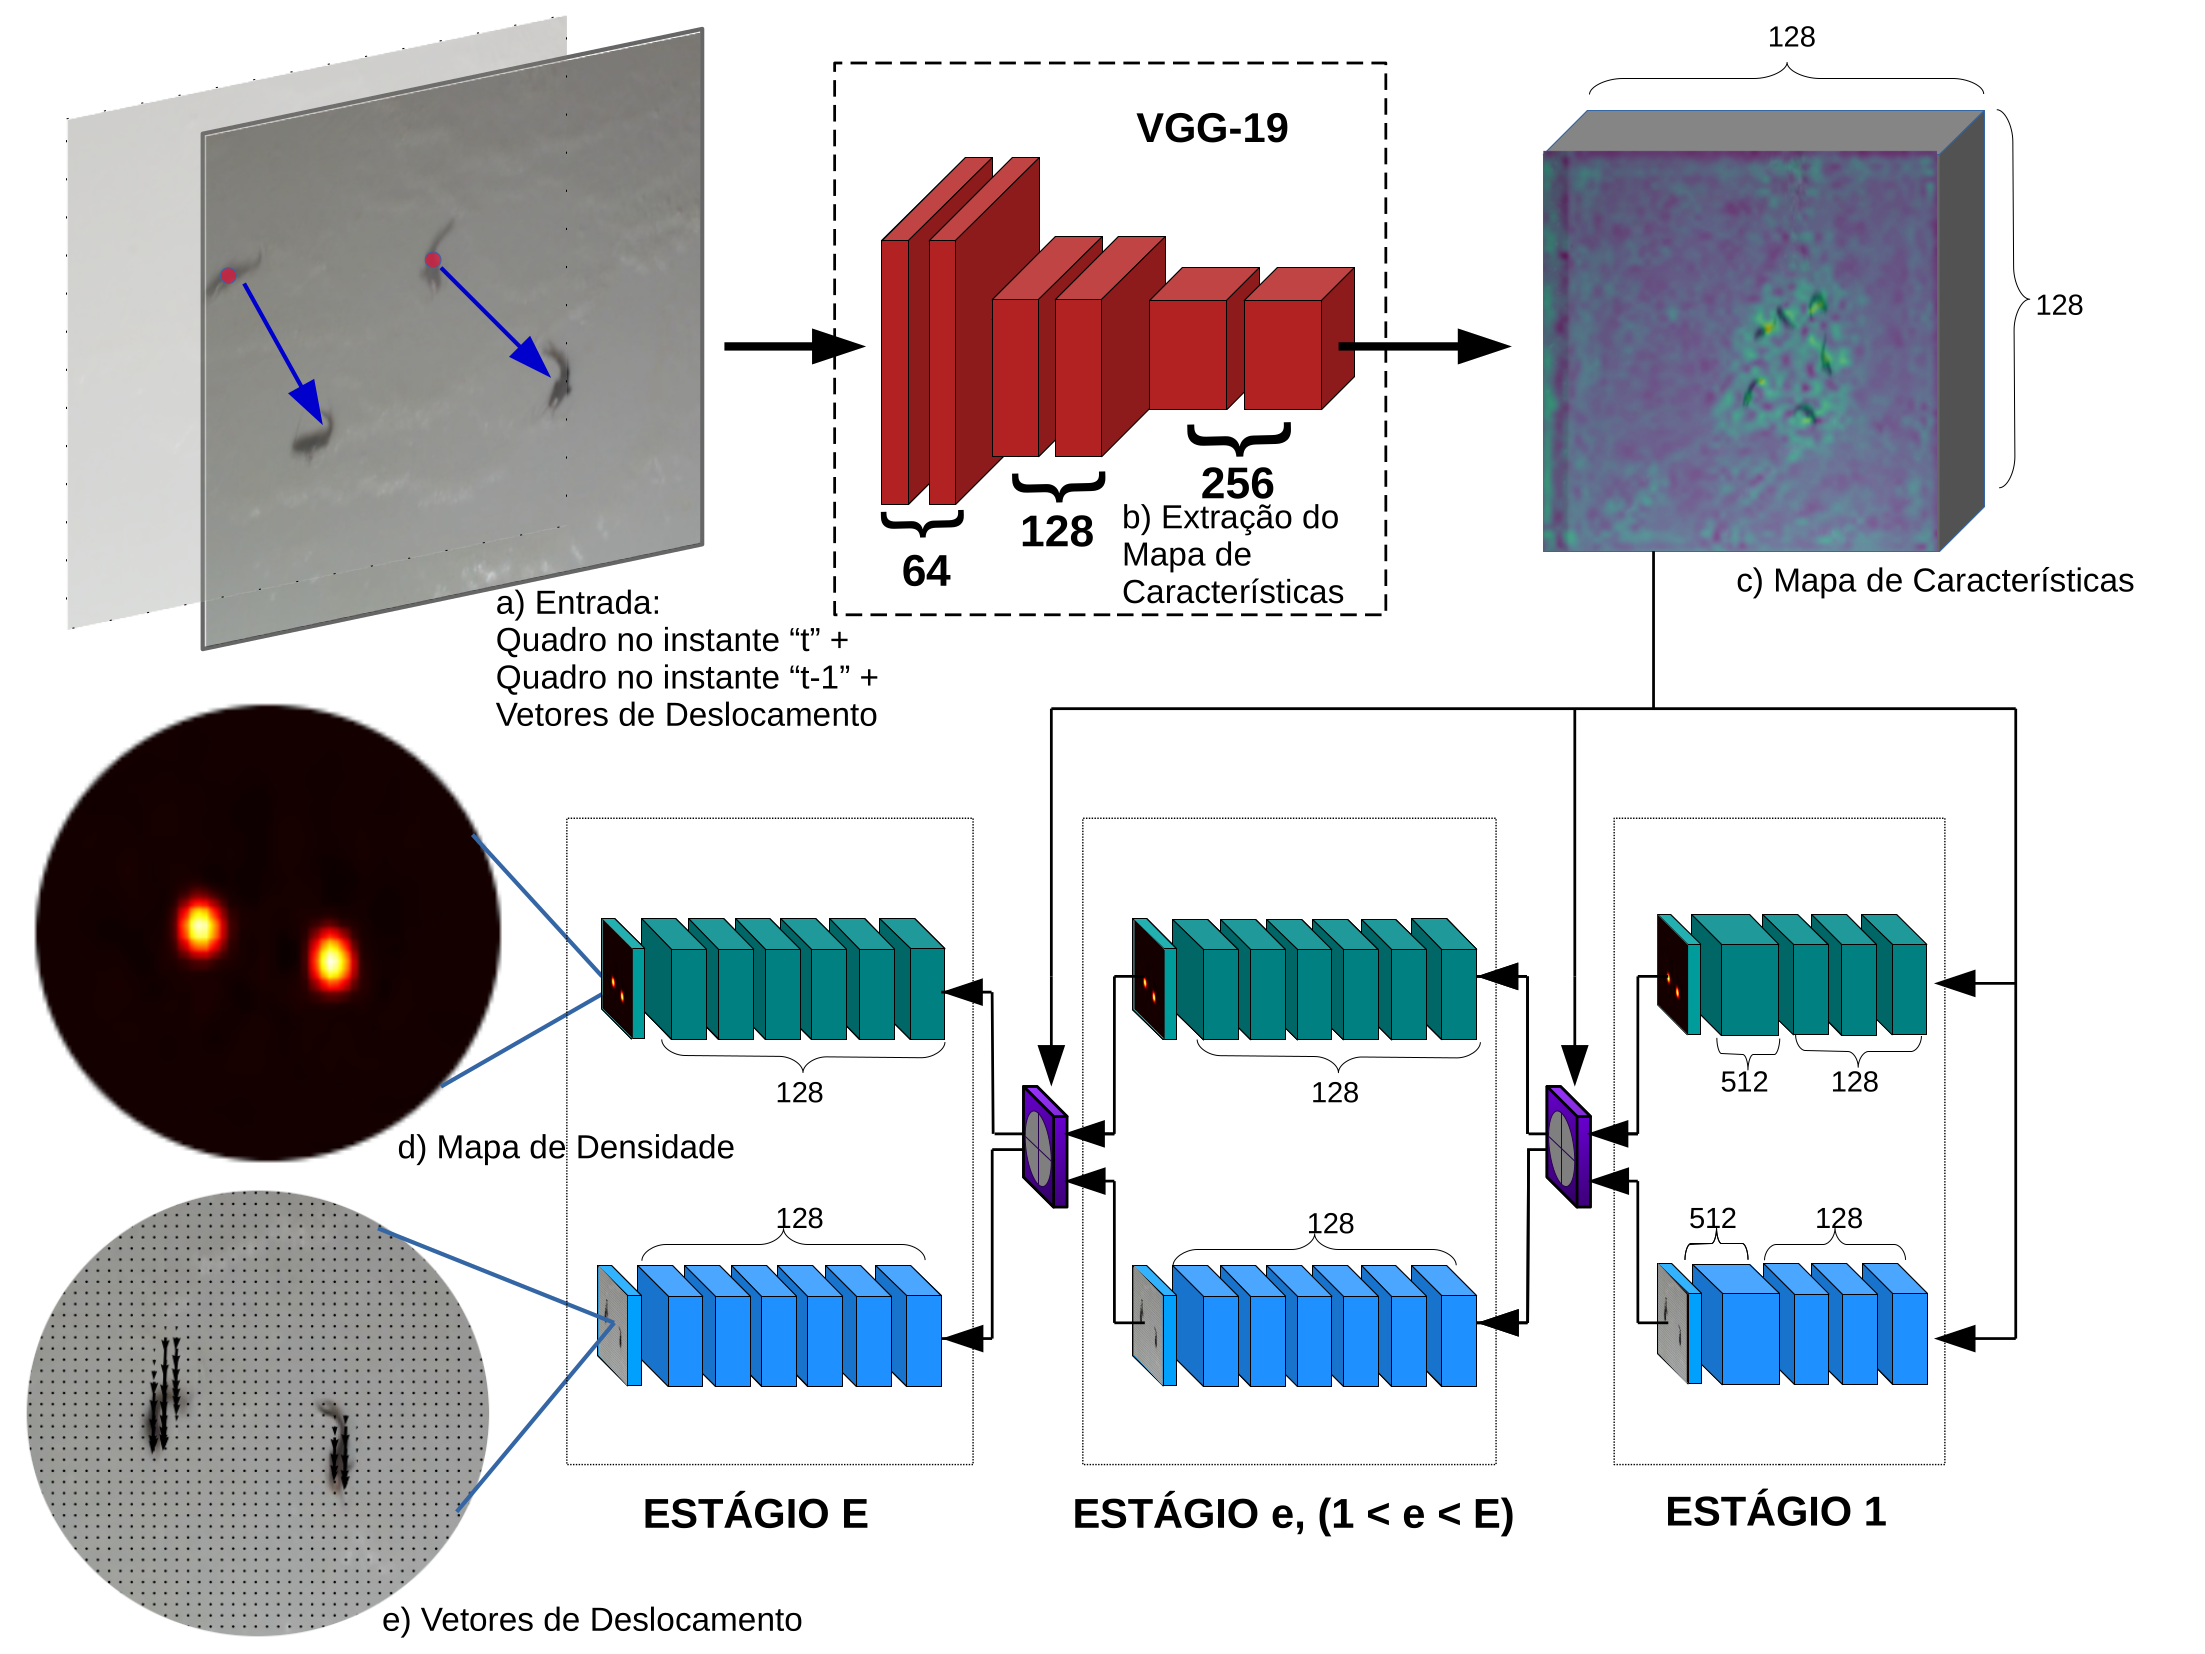
\includegraphics[width=1.06\textwidth]{image/model.png}
	\caption{
	Método proposto recebe o quadro atual $I_{t}$ e o quadro no instante anterior $I_{t-1}$. O resultado da concatenação gera um volume de entrada para a VGG-19. A saída desta arquitetura consiste em um mapa de características inicial. 
	Esse mapa alimenta dois ramos que são responsáveis por realizar as predições do mapa de densidade e de vetores de deslocamento. Cada ramo é composto por uma série de $E$ estágios que refinam a suas predições.
	%Os estágios são as etapas pelas quais o refinamento do mapa de densidade acontece. Cada estágio abrange dois ramos por vez e o resultado de um estágio contém uma grande participação na entrada dos estágios subsequentes. 
	%O mapa de características inicial serve as entradas do estágio 1 até o estágio e. 
	%Os dois ramos de camadas convolucionais são os responsáveis para um melhor ajuste ao modelo: um produz o 1) mapa de densidade e outro os 2) vetores de deslocamento.
	Ambos ramos compartilham as informações para auxiliar na estimação.}
	\label{fig:model} 
\end{figure}
\newpage
\section{Pré-Processamento das Imagens}
\label{sec:Images}

Dada uma imagem $I_t$ no instante $t$ com $w \times h$ pixels, em que $w$ é a largura e $h$ é a altura da imagem, o primeiro pré-processamento consiste em redimensionar todas as imagens para um tamanho fixo de $n \times n$ pixels.
%Em seguida, uma borda de 30 pixels em cada lado da imagem é aplicado.
%Desta forma, um recorte é realizado nas bordas e os peixes são contabilizados apenas na imagem resultante \ref{fig:entrada1}.

%\begin{figure}[!htb]
%	\centering
%	\includegraphics[width=1.0\textwidth]
%	{image/janela2.pdf}
%	\caption{Exemplificação do pré-processamento realizado em cada quadro. Uma borda de 30 pixels em cada lado da imagem é aplicado e os peixes cuja as posições estejam dentre os limites da imagem resultante são contabilizados pelo método.}
%	\label{fig:entrada1} 
%\end{figure} 
%Os ramos são os conjuntos de camadas pelas quais cada $VE$ passa para extração de características. 
%Tendo suas rotinas realizadas por estágios, foram denominados estágio "1", "e = (1<e<E)" e "E". 
%Cada estágio abrange dois ramos, o responsável por extrair os atributos principais dos objetos e o que estima os vetores de deslocamento.
%O mapa de características inicial serve as entradas desde o estágio 1 até o estágio e. 
O método recebe um volume de entrada $V$, resultante da concatenação de um quadro $I_{t}$ no instante $t$ e o quadro anterior $I_{t-1}$, $V = (I_{t},I_{t-1})$, conforme a figura \ref{fig:entrada}.
%o(s) vetor(es) de deslocamento do(s) peixe(s) em um instante anterior $t-1$. 
Sendo $I_{t}$ uma imagem RGB com $512\times512\times3$ pixels e $I_{t-1}$ uma outra imagem do instante anterior com a mesma dimensão, temos que $V$ possui dimensão $ 512\times512\times6$.
%Desta forma temos o volume de entrada $V = (I_{t},I_{t-1})$
%, sendo $I_{t-1}$ os vetores de deslocamento dos peixes de $I_{t-1}$ até $I_{t}$ (Figura \ref{fig:entrada}).
%A CNN VGG-19 (Figura \ref{fig:model}) \cite{VGG} recebe $V$ como entrada e a sua saída consiste em um mapa de características inicial que descreve as informações relevantes da imagem.

\begin{center}
\begin{figure}[!htb]
	\centering
	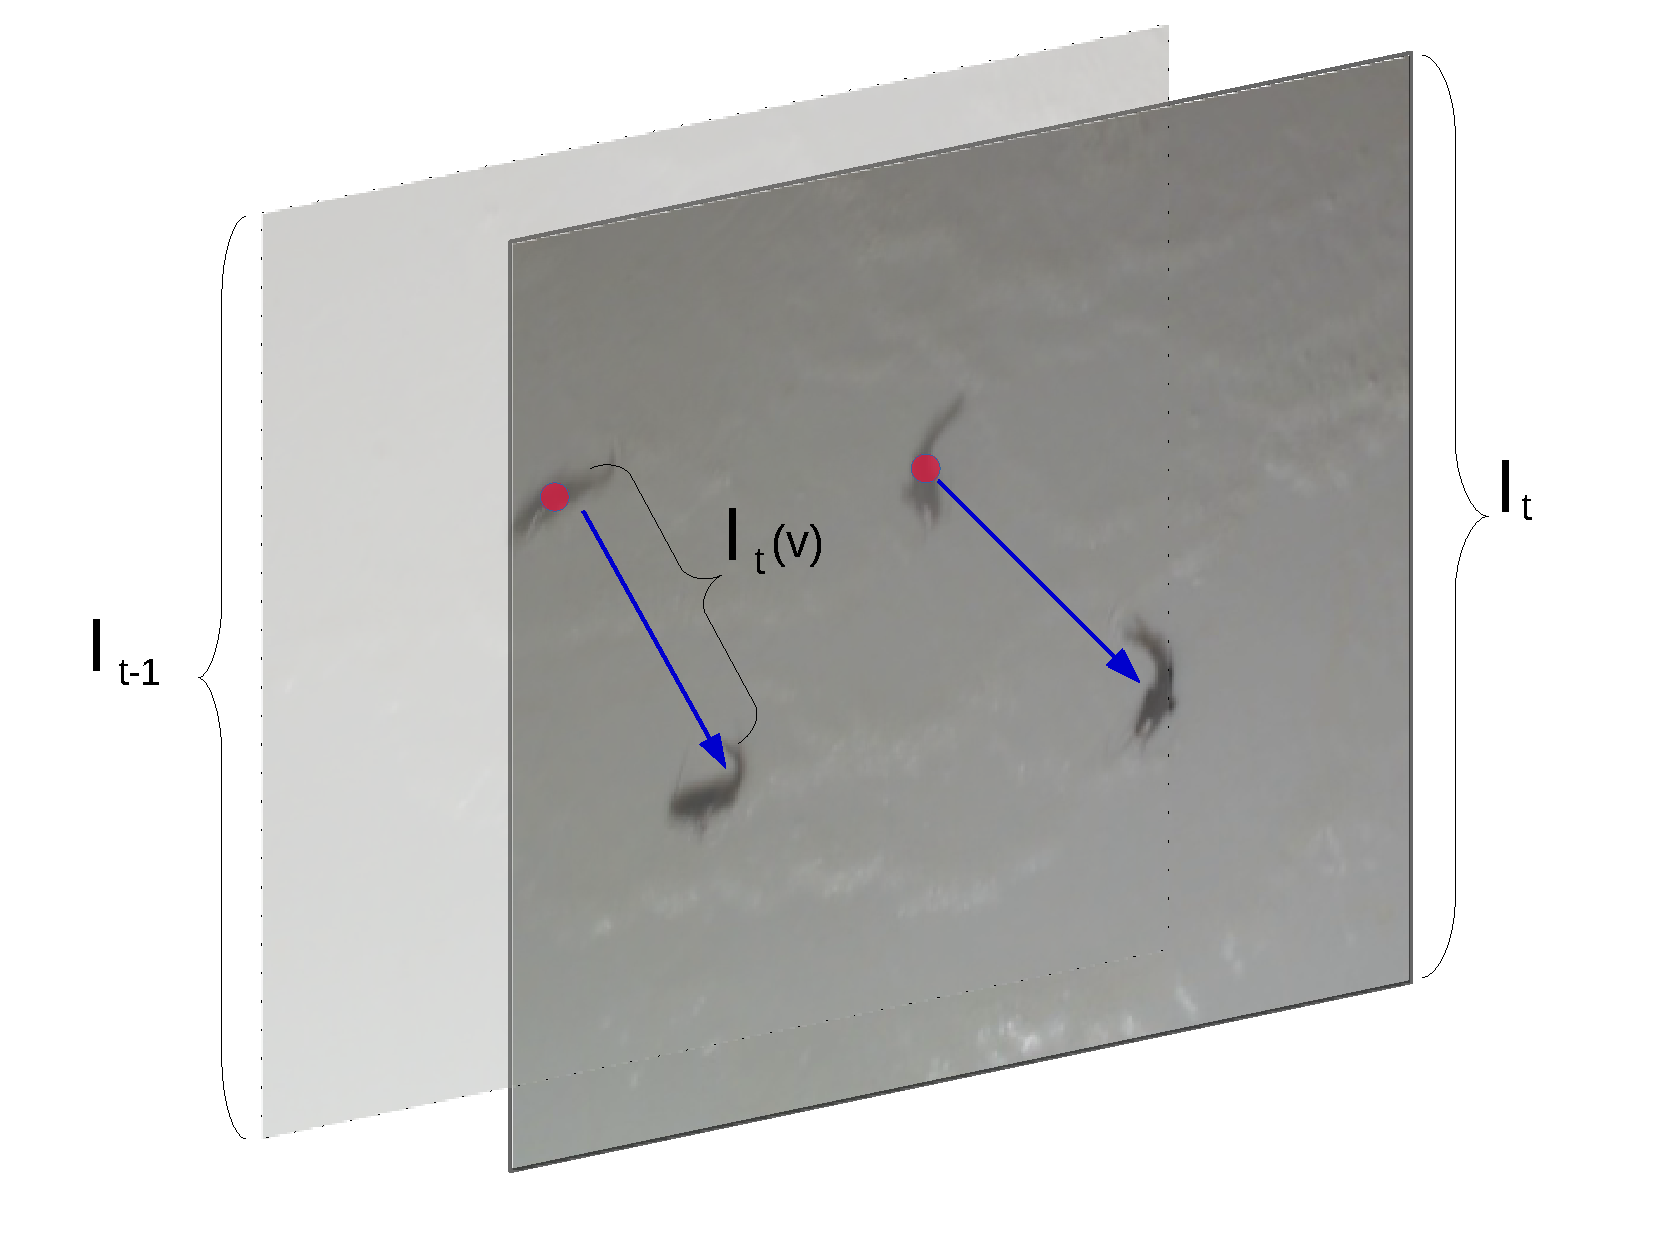
\includegraphics[width=0.9\textwidth]
	{image/VE.pdf}
	\caption{Ilustração do volume de entrada $V$ que consiste na concatenação de um quadro $I_{t}$ e um quadro anterior $I_{t-1}$.}
	\label{fig:entrada} 
\end{figure} 
\end{center}



\section{Extração do Mapa de Características}
   \label{sec:VGG}

Nessa etapa, o volume de entrada $V = (I_{t},I_{t-1})$ é submetido a uma CNN VGGNet \cite{VGG} para obtenção de um mapa de características.
Esse mapa tem como objetivo extrair informações relevantes da imagem de entrada.
A VGGNet mostrou que a profundidade da CNN é um componente importante para o bom desempenho. Os autores da VGG19 apresentaram seis arquiteturas: duas com 11, uma com 13, duas com 16, e uma com 19 camadas \cite{VGG}. A CNN de 19 camadas convolucionais e totalmente conectadas é uma das melhores arquiteturas dentre as propostas pelos autores, sendo uma arquitetura homogênea pois só executa convoluções com campo receptivo $3 \times 3$ e subamostragens $2 \times 2$. A Figura \ref{fig:model} ilustra as camadas da arquitetura VGG19 aplicadas no método proposto.

A entrada da VGG19 consiste em duas imagens RGB com dimensão $512 \times 512 \times 6$, que passa por um pré-processamento inicial no qual é realizada a subtração da cor média de todos os pixels da imagem. Esse processo é repetido para todas as imagens que serão usadas para o treinamento da CNN.
As imagens passam pelas camadas convolucionais que aplicam um filtro de tamanho $3 \times 3$, por ser o menor tamanho capaz de aprender características das quatro direções e do centro durante o processo de convolução. 
O passo de deslocamento do filtro convolucional (\textit{stride}) é de 1 pixel.
O preenchimento com zeros ao redor da imagem é realizado de forma a preservar a dimensão da imagem após a convolução, ou seja, para os filtros de tamanho $3 \times 3$ é usado um preenchimento com zeros de tamanho 1.
Além disso, a função de ativação não-linear ReLu é aplicada após cada camada convolucional.

A amostragem descendente (\textit{Pooling}) é feita através de duas camadas de subamostragens distribuídas no corpo da CNN. Assim, nem todas camadas convolucionais são seguidas de camadas de subamostragens. Os autores usam uma camada de subamostragem máxima com campo receptivo $2 \times 2$ e deslocamento de 2 pixels.
Ao final da primeira etapa, o volume de entrada $V$ é representado por um mapa de características $F$ extraído pelas camadas da VGGNet.
Na Figura \ref{fig:carac} temos a imagem original e o mapa de características obtido através da VGG19.

\begin{figure}[!ht]
	\centering
	\subfloat[Imagem Original]{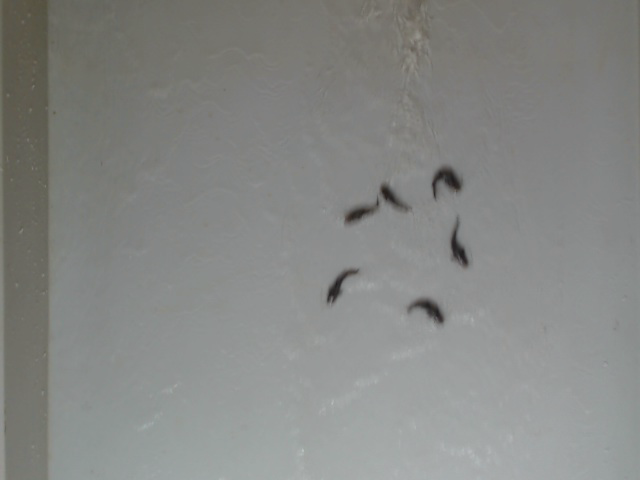
\includegraphics[width=0.5\textwidth]{image/caract.png}}\vspace{0.9cm}
	\subfloat[mapa de características]{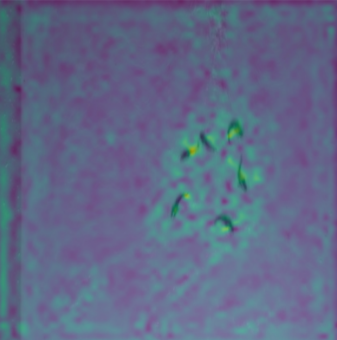
\includegraphics[width=0.37\textwidth]{image/carac.png}}\vspace{0.6cm}
	\caption{\label{fig:carac} Exemplo de um mapa de características predito pela VGG-19.}
\end{figure}  


\section{Estimativa do Mapa de Densidade}
\label{sec:EstimativaDensidade}
Dado o mapa de característica $F$, o primeiro ramo do método proposto estima o mapa de densidade com o objetivo de detectar cada objeto.
Essa predição é realizada por $E$ estágios.
No primeiro estágio (Figura \ref{fig:model} (c)), uma série de camadas convolucionais $\Omega$ geram o mapa de densidade $\hat{C}^1 = \Omega (F)$.
$\Omega$ é uma sequência de cinco camadas convolucionais: três camadas com 128 filtros de tamanho $3 \times 3$, uma camada com 512 filtros de tamanho $1 \times 1$ e uma camada com um único filtro que corresponde ao mapa de densidade.
O segundo ramo responsável pela estimativa dos vetores de deslocamento $\hat{D}^{1}$ estão detalhadas na Seção \ref{sec:EstimativaVetores}. Por enquanto precisamos saber que as estimativas também são utilizados para servir de entrada dos estágios seguintes.

Os estágios refinam as predições do mapa de densidade em etapas sucessivas por $E$ estágios, i.e., $e \in \{1, \dots, E\}$.
Nos estágios subsequentes ao primeiro (Figura \ref{fig:model}), o mapa de características $F$, a estimativa de densidade do estágio anterior $\hat{C}^{e-1}_t$ e as estimativas dos vetores de deslocamento $\hat{D}^{e-1}$ (Seção \ref{sec:EstimativaVetores}) são concatenados e usados para produzir um mapa de densidade refinado $\hat{C}^e = \Psi(F, \hat{C}^{e-1}, \hat{D}^{e-1})$.
A concatenação de diferentes informações auxilia no apendizado do método e espera-se que a informação de deslocamento ajude na detecção dos objetos no quadro atual.
No refinamento, $\Psi$ é uma sequência de sete camadas convolucionais: cinco camadas com 128 filtros de tamanho $7 \times 7$, uma camada com 128 filtros de tamanho $1 \times 1$ e uma camada com um único filtro que corresponde ao mapa de densidade. 



%\begin{figure}[!ht]
%	\centering
%	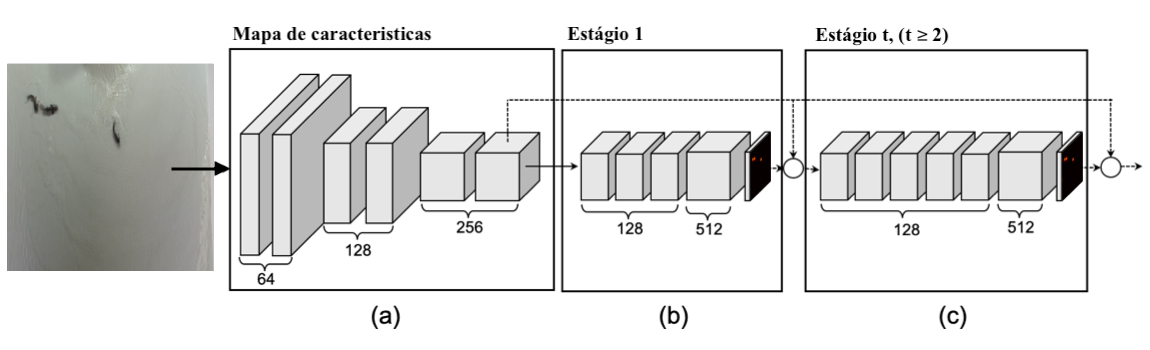
\includegraphics[width=1.0\textwidth]{image/cnn.png}
%	\caption{\label{fig:cnn} CNN usada para predição do mapa de confiança. Bloco inicial (a) é usado para extrair um mapa de recursos da imagem de entrada. Este mapa de recursos é usado como entrada para o primeiro estágio (b). A concatenação do mapa de características e o mapa predito do estágio anterior são usados como entrada para os estágios restantes.}
%\end{figure}  

Para treinar os estágios, a função de perda (Equação \ref{eq:loss}) é aplicada no final de cada estágio comparando a predição do método $\hat{C}^{e}$ com as anotações realizadas por um especialista $C$.
Esta supervisão intermediária aborda o problema do gradiente de desaparecimento, como mostrado em \cite{Cao2017}.
%Como o tamanho do mapa de densidade estimado é menor que o tamanho da imagem, o mapa de densidade \textit{ground truth} é gerado com o tamanho da saída da CNN $[l_F \times l_F]$.

\begin{equation}
f^{e} = \sum_p \parallel C(p) - \hat{C}^{e}(p)\parallel^2_2,
\label{eq:loss}
\end{equation}
onde $C$ é o \textit{ground truth} do mapa de densidade do quadro $t$ gerado de acordo com a Seção \ref{sec:geracao_mapa}. Por fim, a função de perda global é dada pela soma de todos os estágios:

\begin{equation}
f = \sum_{e=1}^{E} f^{e}
\end{equation}

\subsection{Geração do \textit{Ground Truth} do Mapa de Densidade}
\label{sec:geracao_mapa}

Dadas as posições $L = [\{l^1, l^2, \dots, l^K \} \mid \forall \: l^k = (x_k, y_k)]$ de $K$ objetos em um quadro $I_t$, o mapa de confiança (\textit{ground truth}) $C$ é obtido colocando-se um núcleo Gaussiano 2D em cada posição dos objetos. 
Para obter $C$, um mapa de confiança $C^k$ é primeiro calculado para cada objeto $k \in [1, K]$.
O valor de cada posição $p \in \Re^2$ em $C^k$ é definido como:

\begin{equation}
C^k(p) = \exp \left(- \frac{\| p - l^k \|^2_2}{\sigma^2}\right),
\end{equation}
onde $\sigma$ corresponde a largura dos picos que representa cada objeto.
%onde $\sigma = \{\sigma_{min}, \dots ,\sigma_{max}\}$ sendo $\sigma_i \in \mathbb{R}^*_+$. $\sigma_{max}$ aponta a largura da base dos picos e $\sigma_{min}$ recebe um valor mínimo que indica a largura das extremidades. Assim $\sigma$ limita o tamanho dos picos para estimar o tamanho médio de cada objeto.

%\begin{equation}
%    \label{eq:sigma}
%    \sigma = \sum_{i=s_{min}}^{s_{max}} s_{i}
%\end{equation}

%onde $\sigma = \sum_{i=m}^{s_i} s_{max}$ e $s_i \in \mathbb{R}^*_+$.


%Idealmente, $\sigma$ é proporcional à largura média do objeto.
O mapa de confiança $C$ é obtido pela agregação dos mapas individuais via operador máximo:

\begin{equation}
C(p) = \max_{1<k<K} C^k(p).
\end{equation}

A Figura \ref{fig:sigma} ilustra o mapa de confiança para uma imagem e dois valores de $\sigma$.
A primeira imagem mostra as posições dos objetos em pontos vermelhos que foram anotados pelo especialista.
As próximas duas imagens apresentam os mapas de confiança para $\sigma = 1.5$ e $2.5$, respectivamente.
Por fim, usamos o mapa de confiança \textit{ground truth} para treinar a abordagem proposta.

\begin{figure}[!ht]
	\centering
	\subfloat[Imagem Original]{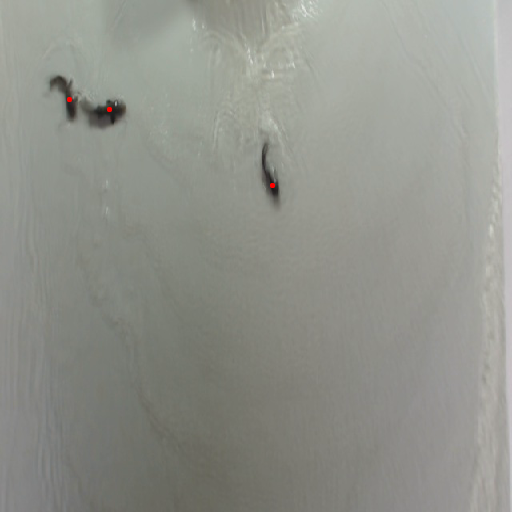
\includegraphics[width=0.3\textwidth]{image/sigmas/frame001018Ponto.png}}\vspace{0.2cm}
	\subfloat[$\sigma = 1.5$]{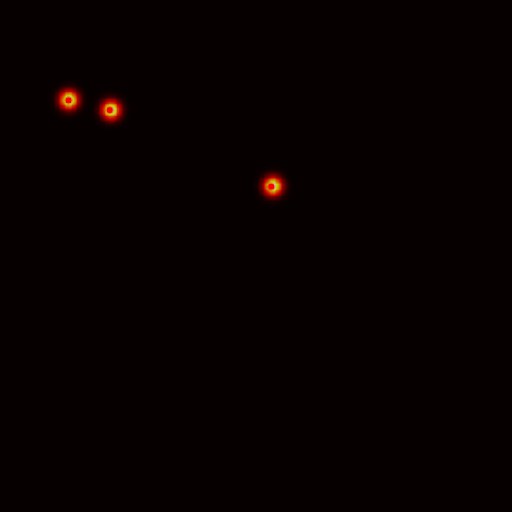
\includegraphics[width=0.3\textwidth]{image/sigmas/frame001018_label_1_5.png}}\vspace{0.2cm}
	\subfloat[$\sigma = 2.5$]{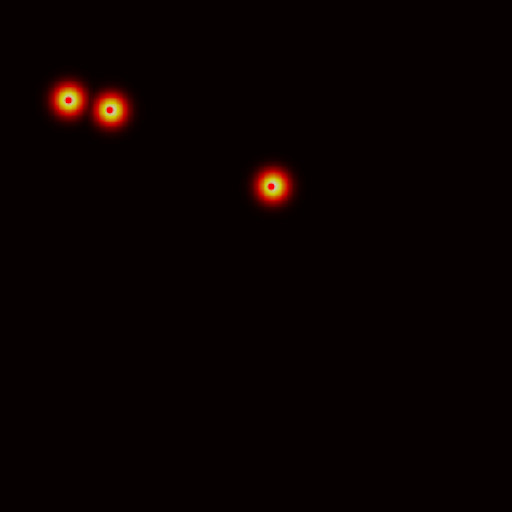
\includegraphics[width=0.3\textwidth]{image/sigmas/frame001018_label_2_5.png}}
	\caption{\label{fig:sigma} Exemplo de uma cena e seu mapa de confiança correspondente para diferentes valores de $\sigma$.}
\end{figure}  


\section{Estimativa dos Vetores de Deslocamento}
\label{sec:EstimativaVetores}

O segundo ramo do método proposto (Figura \ref{fig:model} (d)) possui camadas convolucionais com os mesmos parâmetros do primeiro ramo.
%Entretanto, a útilma camada de cada estágio produz um vetor un
Entretanto, a última camada de cada estágio produz a estimativa do deslocamento em x e y.
O primeiro estágio possui uma série de camadas convolucionais $\Omega$ que geram os vetores de deslocamento $\hat{D}^{1} = \Omega (F)$ para o quadro $t$.

Nos demais estágios, o mapa de características $F$, o mapa de densidade $\hat{C}^{e-1}$ (Seção \ref{sec:EstimativaDensidade}) e a estimativa do estágio anterior $\hat{D}^{e-1}$, são concatenados e usados para produzir os vetores de deslocamento refinado $\hat{D}^{e} = \Psi(F,\hat{C}^{e-1}, \hat{D}^{e-1}$). 
$\Psi$ é uma sequência de sete camadas convolucionais conforme o primeiro ramo.

Para treinar os estágios dos vetores de deslocamento, a função de perda (Equação \ref{eq:loss2}) é aplicada no final de cada estágio.

\begin{equation}
f^{e} = \sum_p \parallel D(p) - \hat{D}^{e}(p)\parallel^2_2,
\label{eq:loss2}
\end{equation}
onde $D$ é o \textit{ground truth} dos vetores de deslocamento do quadro $t$ gerado de acordo com a Seção \ref{sec:geracao_mapa2}. Por fim, a função de perda global é dada por:

\begin{equation}
f = \sum_{e=1}^{E} f^{e}
\end{equation}

\subsection{Geração do \textit{Ground Truth} do Vetor de Deslocamento}
\label{sec:geracao_mapa2}

%Dada a posição $l^k_t \in L$ (Seção \ref{sec:geracao_mapa}) de um objeto $k$ presente em um quadro $t$, campos vetoriais são estimados, onde $l_{t,n} \in \mathbb{R}^{w\times h\times2}$, $f \in \{1...N\}$, cada local da imagem em $L_t$ codifica um vetor 2D.

Considere $l_t^k$ como a posição de um objeto $k$ no quadro $t$ e $l_{t-1}^k$ sua posição no quadro anterior.
%Considere a posição de um objeto k na imagem como $l_t^k$ e a sua posição no quadro anterior  
O vetor de deslocamento do objeto $k$ é um vetor que aponta de $l^k_{t-1}$ até $l^k_{t}$, conforme a Figura \ref{fig:vetor}.
Para a construção dos vetores de deslocamento densos, isto é, para cada pixel da imagem, um conjunto de pixels $\rho$ ao redor do vetor de deslocamento principal é obtido.
Todos os pixels cuja a distância para o vetor de deslocamento for menor ou igual a um é considerado nesse conjunto.
%Considere a posição de um único objeto presente em um quadro, sendo $x_{i2}$ o \textit{Ground Truth} e a posição de onde ele se encontrava no quadro anterior sendo $x_{i1}$. 
%Sendo $\rho$ o conjunto de pixels referentes a $l^k_{t}$. 
Cada pixel $p \in \rho$ armazena um vetor unitário $v$ com a mesma direção do deslocamento de $t-1$ para $t$ do objeto $k$, sendo $v = (l^k_{t-1} - l^k_{t})/\|(l^k_{t-1} - l^k_{t})\|_2$.
Os pixels restantes recebe um vetor nulo. 
O mesmo procedimento é realizada para todos os objetos $k$ no quadro atual e um mapa denso de vetor de deslocamento $D$ é obtido para treinamento do método proposto.

\begin{figure}[!htb]
	\centering
 	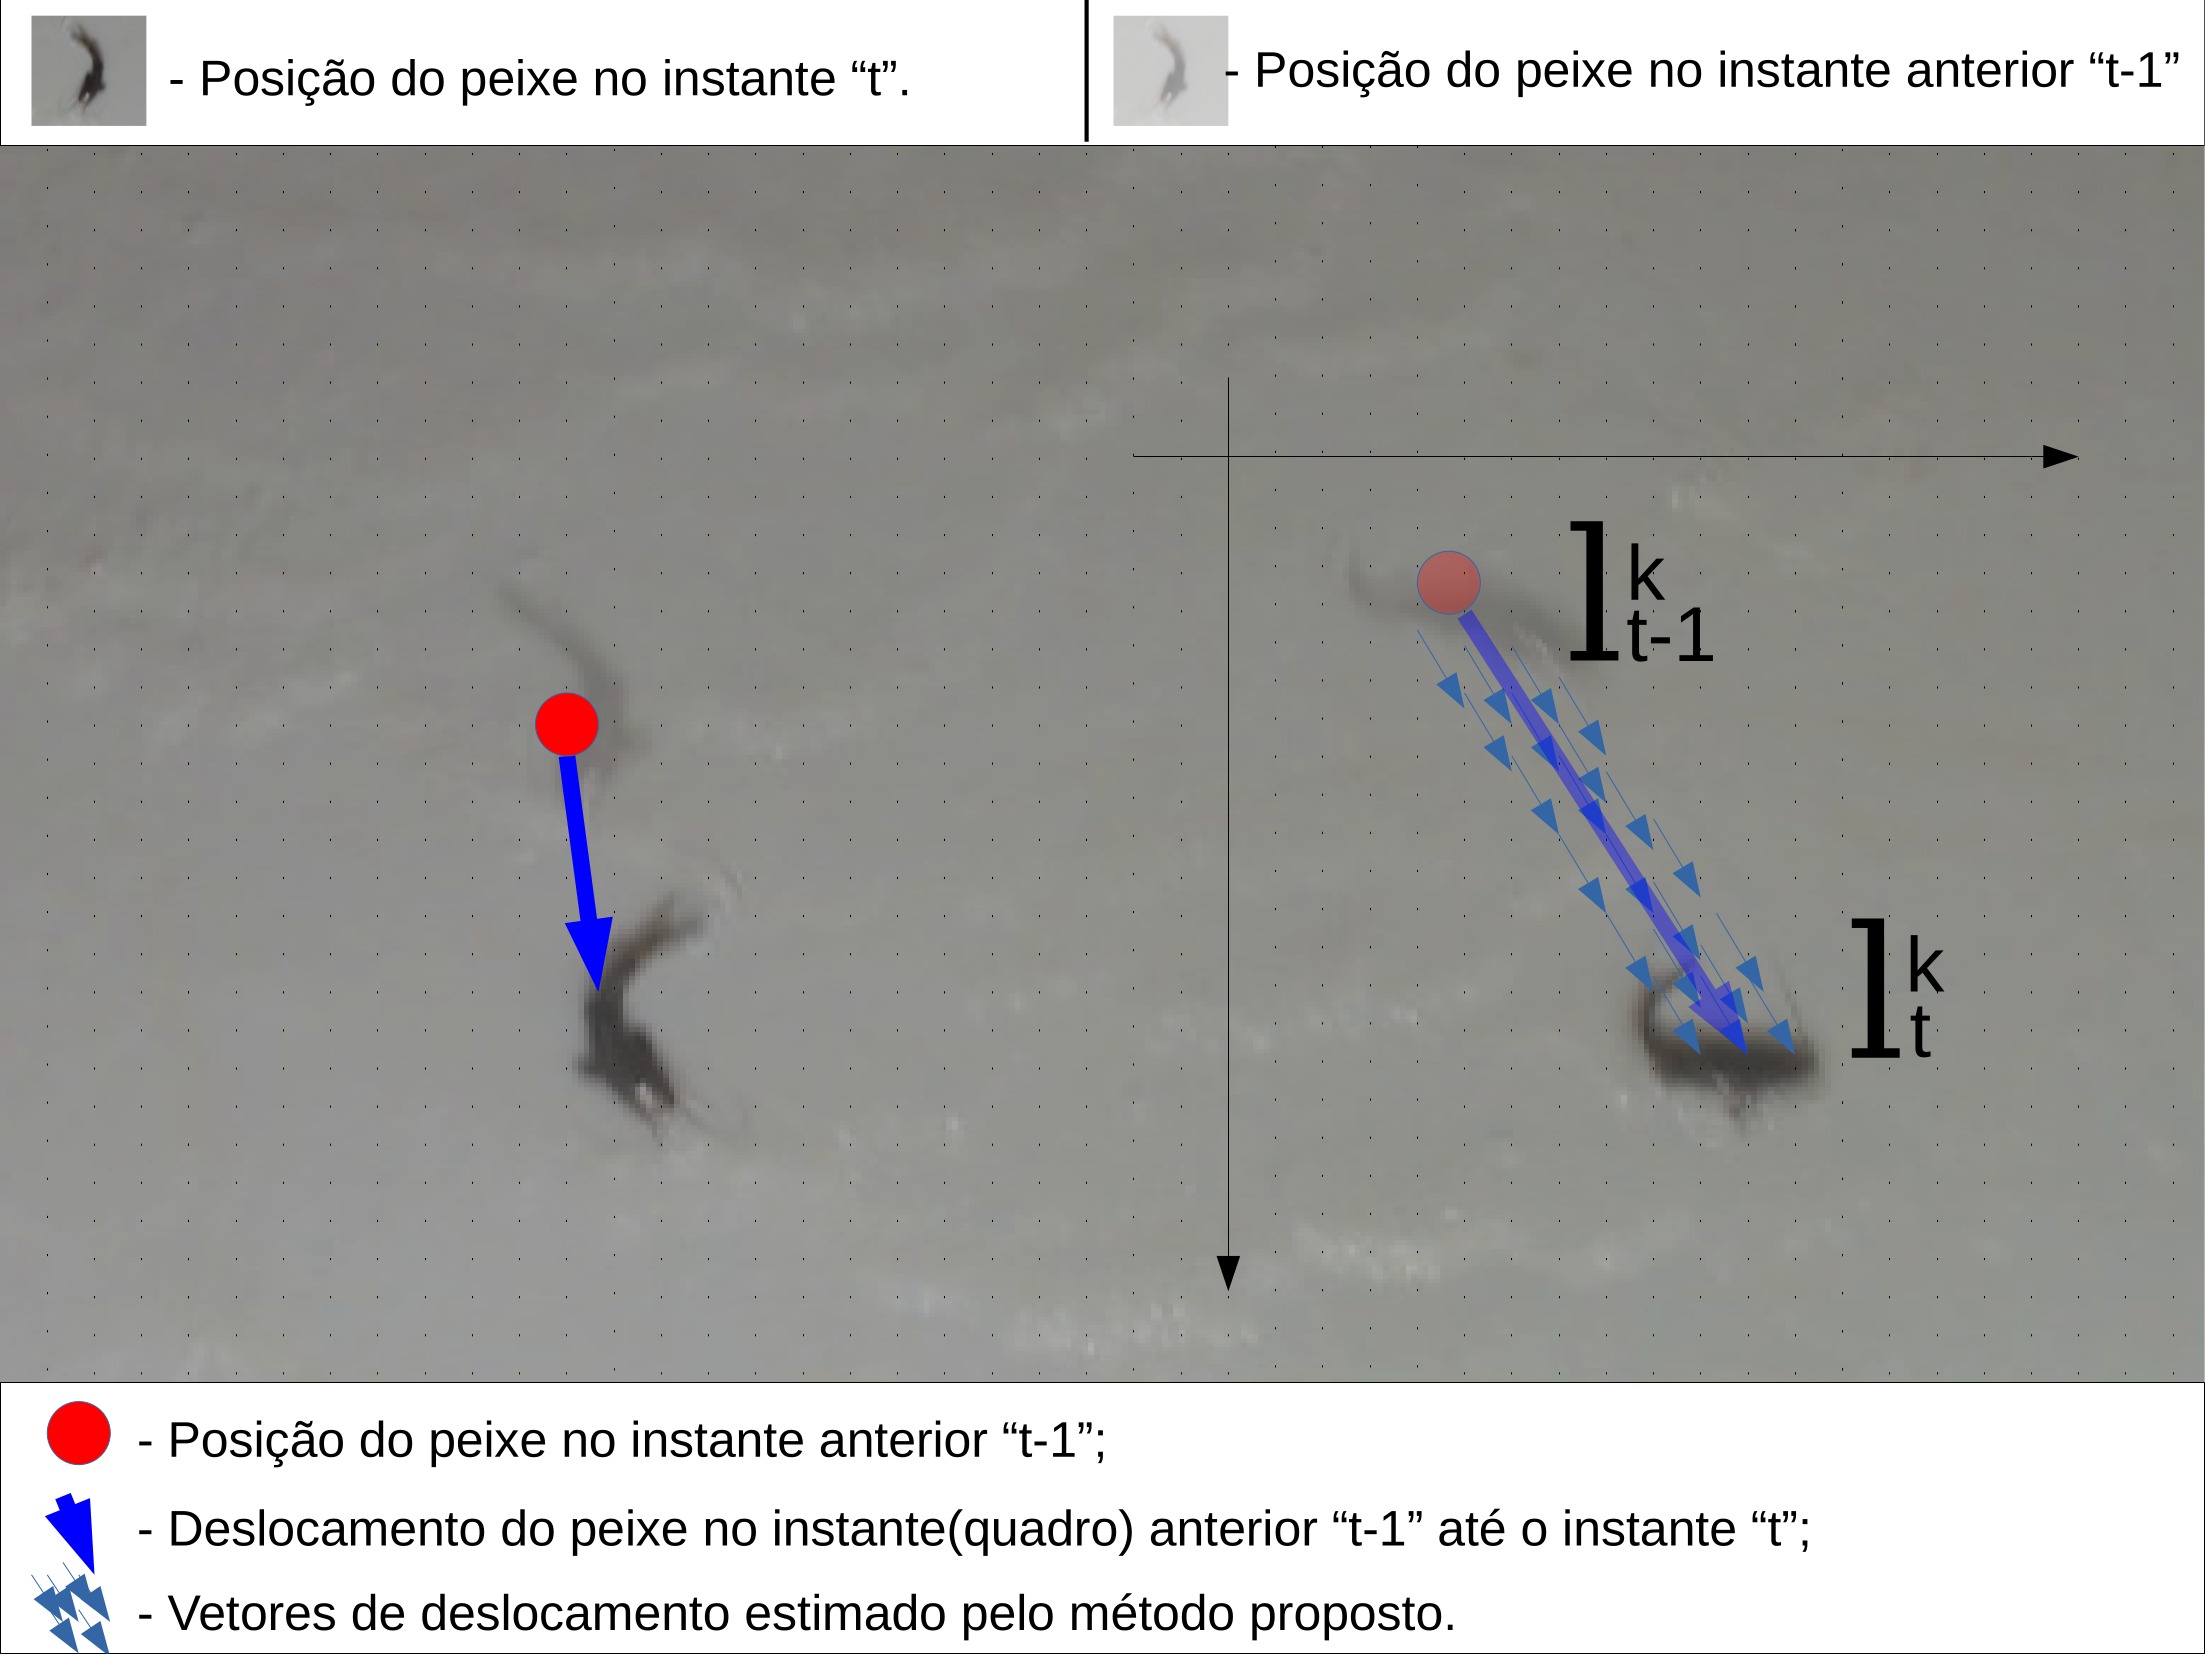
\includegraphics[width=.9\textwidth]{image/VD.png}\vspace{0.2cm}
	\caption{\label{fig:vetor} Ilustração de um vetor para um objeto em quadro.}
\end{figure} 


A Figura \ref{fig:vetores} mostra os alevinos na cor branca, os pontos na cor azul apontam a posição dos alevinos no quadro atual $I_t$ e os pontos na cor vermelho mostram as localizações no quadro anterior $I_{t-1}$. Nas imagens da Figura \ref{fig:vetores2} temos a ilustração dos vetores estimados, sendo estimado um vetor para cada pixel que representa o objeto de interesse.
%As figuras mostram os pontos do quadro anterior quando apenas dois \textit{frames} são utilizados, quando o número de quadros anteriores é superior a um, os quadros atuais apontam um vetor com as posições anteriores de cada filhote.

\begin{figure}[h]
	\centering
	\subfloat[]{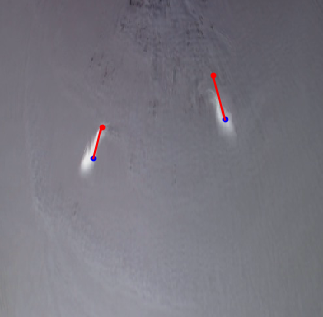
\includegraphics[width=0.3\textwidth]{image/frame000089.png_tracking.png}}\vspace{0.1cm}
	\subfloat[]{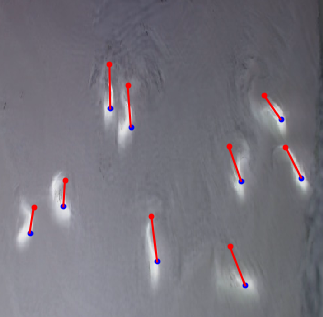
\includegraphics[width=0.3\textwidth]{image/frame000126.png_tracking.png}}\vspace{0.2cm}
	\subfloat[]{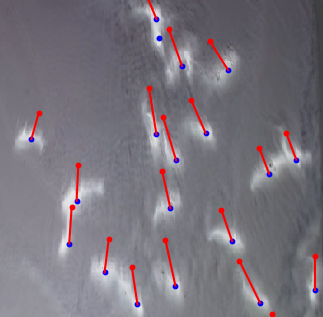
\includegraphics[width=0.3\textwidth]{image/frame000176.png_tracking.png}}
	\caption{\label{fig:vetores} Exemplos das localizações nos vetores}
\end{figure} 

\begin{figure}[h]
	\centering
	\subfloat[]{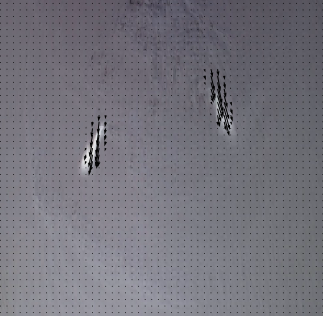
\includegraphics[width=0.3\textwidth]{image/frame000089.pngquiver_t.png}}\vspace{0.1cm}
	\subfloat[]{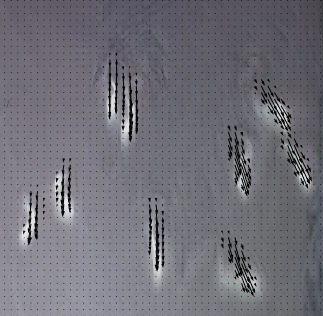
\includegraphics[width=0.3\textwidth]{image/frame000126.pngquiver_t.png}}\vspace{0.2cm}
	\subfloat[]{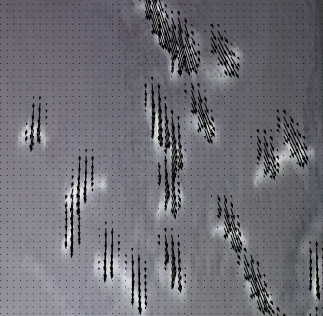
\includegraphics[width=0.3\textwidth]{image/frame000176.pngquiver_t.png}}
	\caption{\label{fig:vetores2} Ilustração dos vetores estimados pelo segundo ramo apresentado, para cada pixel de cada objeto.}
\end{figure} 

\newpage
\section{Localiza\c{c}\~{a}o dos Objetos pelo Mapa de Densidade}

A localização dos objetos é obtida dos picos (máximo local) do mapa de densidade predito do último estágio $\hat{C^E}$.
Um local $p=(x_p, y_p)$ é um máximo local se $\hat{C^E}(p) > \hat{C^E}(v)$ para todos os vizinhos $v$.
Consideramos a vizinhança de 4 pixels para todos os locais $p = (x_p, y_p)$, ou seja, $v = (x_p \pm 1, y_p)$ ou $(x_p, y_p \pm 1)$.

Para evitar ruído, os picos precisam ser separados por pelo menos $\delta$ pixels.
Isso impede que dois alevinos sejam detectados muito próximos uns dos outros.
Além disso, um pico deve ter uma confiança maior que um limite $\tau$.
Após experiências preliminares, usamos $\delta = 10$ e $\tau = 0.2$.
A Figura \ref{fig:heatmap} mostra um exemplo tridimensional do mapa de confiança, onde a largura e a altura são as dimensões da imagem e os picos azuis representam as regiões com máxima confiança local.

\begin{figure}[h]
	\centering
	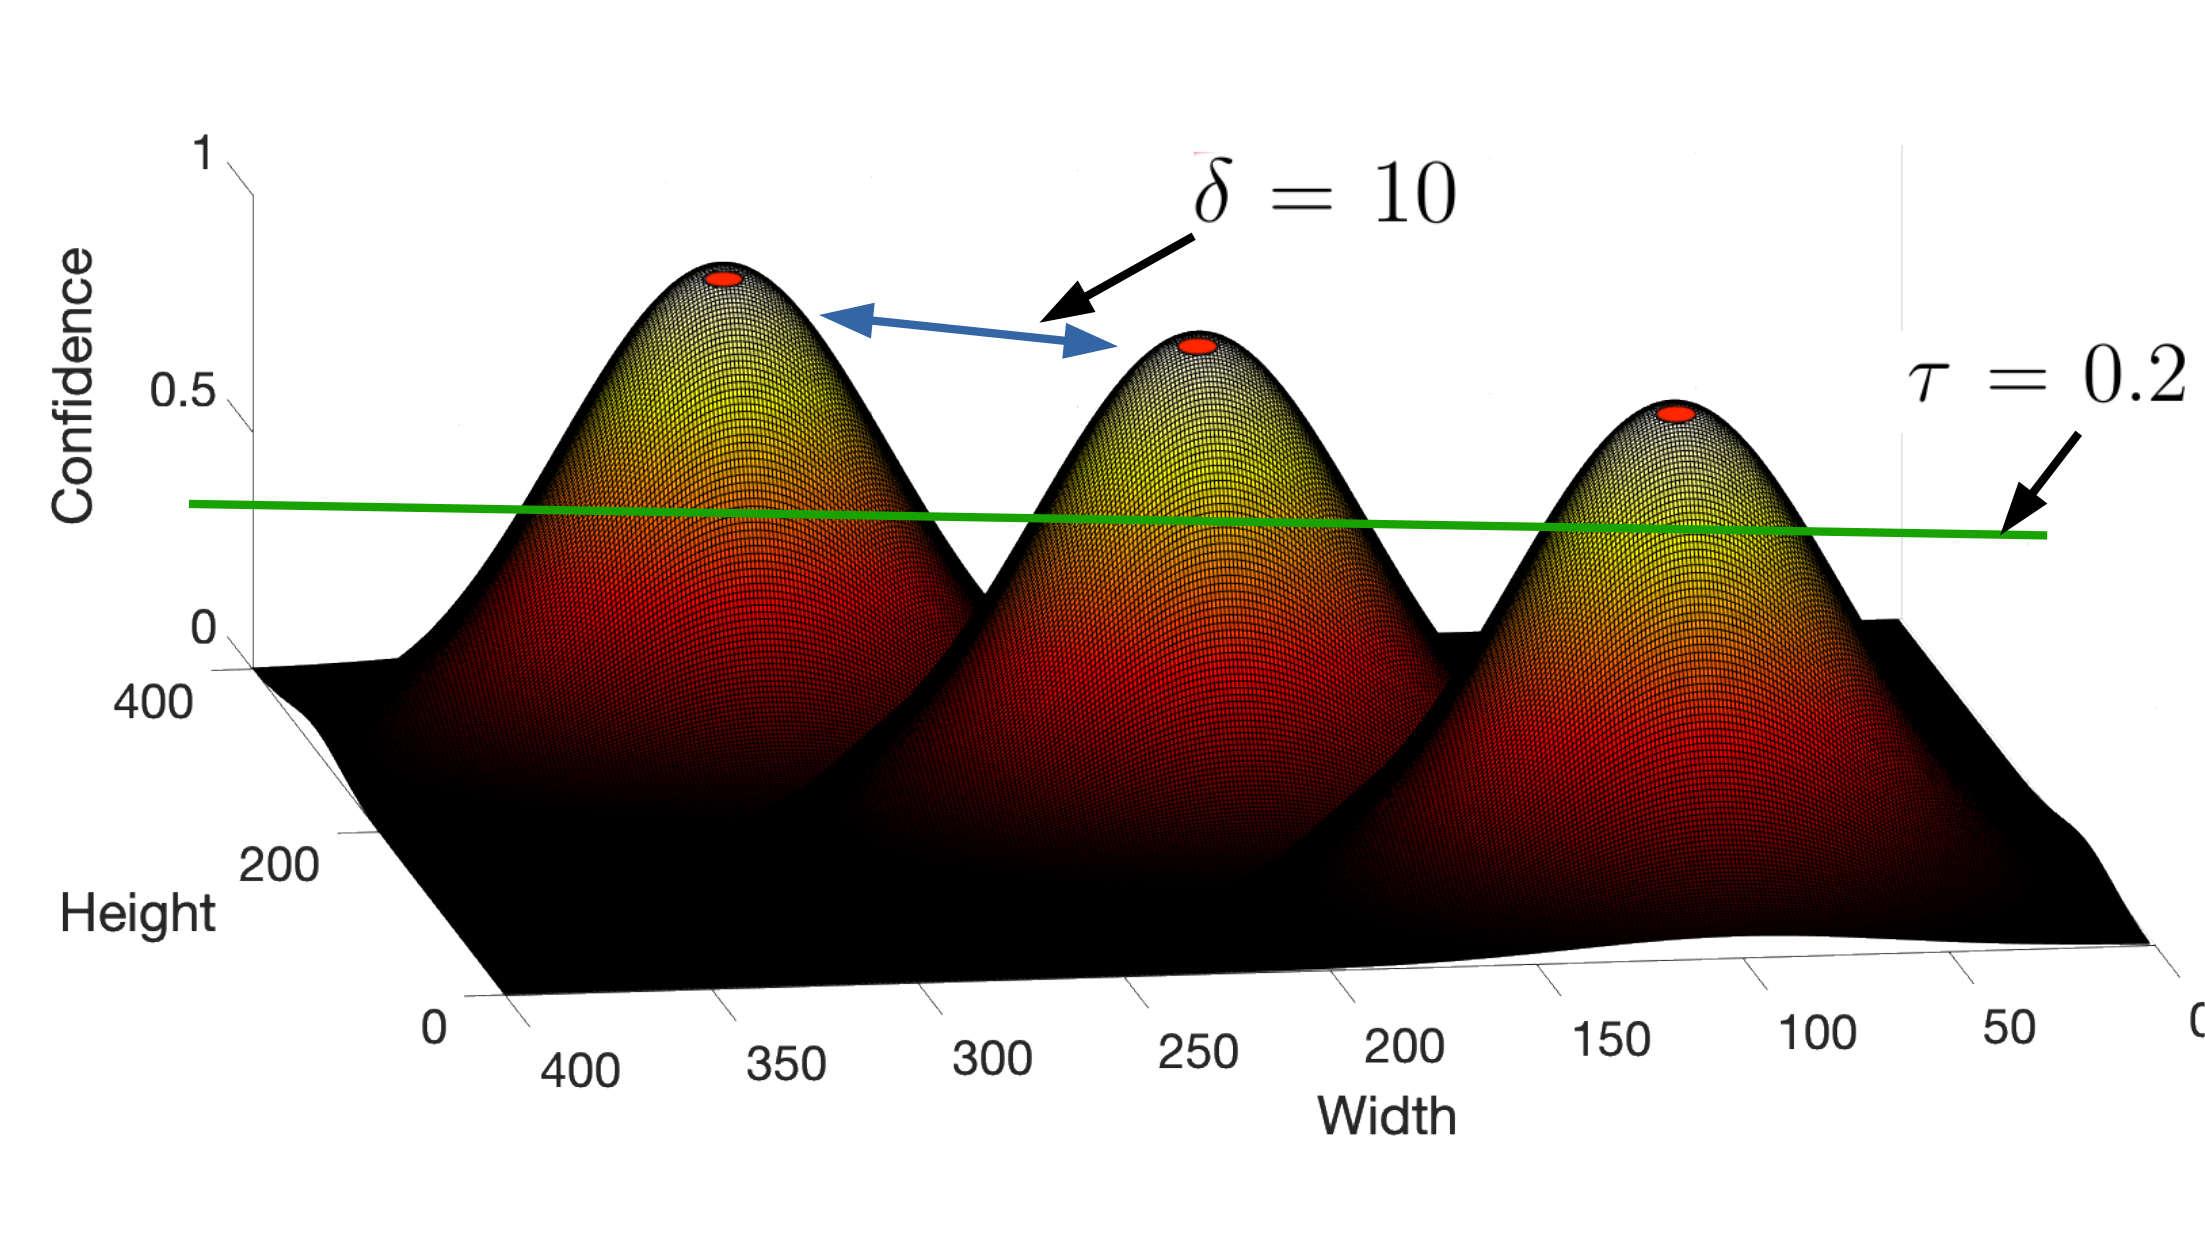
\includegraphics[width=.6\columnwidth]{image/heatmap2.png}
	\caption{Exemplo do mapa de confiança em três dimensões.}
	\label{fig:heatmap}
\end{figure}  

\label{chap:ranking}
